\part{Memory Management}

\chapter{An Overview to Memory Management in Zeke}

In this chapter we will briefly introduce the architectural layout of memory
management in Zeke. Zeke as well as most of major operating systems divides
its memory management and mapping to several layers to hide away any hardware
differences and obscurities. In Zeke these layers are \ac{MMU} \acs{HAL} that
abstracts the hardware, \verb+dynmem+ handling the dynamic allocation of
contiguous blocks of memory and \verb+kmalloc+ that allocates memory for the
kernel itself, and probably most importantly \verb+vralloc/buf/bio+ subsystem
that's handling all allocations for processes and IO buffers. Relations between
different kernel subsystems using and implementing memory management are shown
in figure \ref{figure:vmsubsys}.

\begin{figure}
\begin{verbatim}
U                      +---------------+
S                      |    malloc     |
R                      +---------------+
------------------------------ | -----------
K   +---------------+  +---------------+
E   |    kmalloc    |  |     proc      |
R   +---------------+  +---------------+
N           |     /\    |      |
E           |     |    \/      |
L  +-----+  |  +---------+   +----+
   | bio |--|--| vralloc |---| vm |
   +-----+  |  +---------+   +----+
            |     |            |
           \/    \/            \/
    +---------------+     +----------+
    |    dynmem     |-----| ptmapper |
    +---------------+     +----------+
            |                  |
           \/                  |
    +---------------+          |
    |    mmu HAL    |<----------
    +---------------+
            |
    +-----------------------+
    | CPU specific MMU code |
    +-----------------------+
----------- | ------------------------------
H   +-------------------+
W   | MMU & coProcessor |
    +-------------------+
\end{verbatim}
\caption{Memory management related subsystems and main users of the subsystems
         in Zeke.}
\label{figure:vmsubsys}
\end{figure}

\begin{itemize}
  \item \verb+kmalloc+  - is a kernel level memory allocation service, used
                        solely for memory allocations in kernel space.
  \item \verb+vralloc+  - VRAlloc is a memory allocator targeted to allocate
                        blocks of memory that will be mapped in virtual
                        address space of a processes, but it's widely used
                        as a generic allocator for medium size allocations,
                        it returns a \verb+buf+ structs that are used to
                        describe the allocation and its state.
  \item \verb+bio+      - is a IO buffer system, mostly compatible with the
                        corresponding interface in BSD kernels,
                        utilizing vralloc and buf system.
  \item \verb+dynmem+   - is a dynamic memory allocation system that allocates
                        \& frees contiguous blocks of physical memory (1 MB).
  \item \verb+ptmapper+ - owns all statically allocated page tables
                        (particularly the master page table) and regions,
                        and it is also used to allocate new page tables from
                        the page table region.
  \item \verb+vm+       - vm runs various checks on virtual memory access,
                        copies data between user land, kernel space and
                        allocates and maps memory for processes, and wraps
                        memory mapping operations for proc and \acs{bio}.
  \item mmu HAL -       is an interface to access MMU, provided by \verb+mmu.h+
                        and \verb+mmu.c+.
  \item CPU specific MMU code is the module responsible of configuring the
        physical MMU layer and implementing the HW interface provided by
        \verb+mmu.h+
\end{itemize}

\begin{table}
\caption{The memory map of Zeke running on BCM2835.}
\label{table:bcm_memmap}
\begin{tabular}{l|c|l}
Address                     &   & Description                   \\
\hline
\textbf{Interrupt Vectors}  &   &                               \\
0x0 - 0xff                  &   & Not used by Zeke              \\
0x100  - 0x4000             & L & Typical placement of ATAGs    \\
\textbf{Priv Stacks}        &   &                               \\
0x1000 - 0x2fff             & Z & Supervisor (SWI/SVC) stack    \\
0x3000 - 0x4fff             & Z & Abort stack                   \\
0x5000 - 0x5fff             & Z & IRQ stack                     \\
0x6000 - 0x6fff             & Z & Undef stack                   \\
0x7000 - 0x7fff             & Z & System stack                  \\
0x8000 - 0x3fffff           & Z & Kernel area (boot address)    \\
0x00400000-                 & Z & Page Table                    \\
0x007FFFFF                  &   & Area                          \\
0x00800000                  & Z & Dynmem                        \\
0x00FFFFFF                  &   & Area                          \\
-                           &   &                               \\
\textbf{Peripherals}        &   &                               \\
0x20000000 -                &   &                               \\
\textit{Interrupts}         &   &                               \\
0x2000b200                  & B & IRQ basic pending             \\
0x2000b204                  & B & IRQ pending 1                 \\
0x2000b20c                  & B & IRQ pending 2                 \\
0x2000b210                  & B & Enable IRQs 1                 \\
0x2000b214                  & B & Enable IRQs 2                 \\
0x2000b218                  & B & Enable Basic IRQs             \\
0x2000b21c                  & B & Disable IRQs 1                \\
0x2000b220                  & B & Disable IRQs 2                \\
0x2000b224                  & B & Disable Basic IRQs            \\
- 0x20FFFFFF                & B & Peripherals
\end{tabular}

\begin{tabular}{l|l}
\multicolumn{2}{c}{} \\
\multicolumn{2}{c}{Legends} \\
\hline
Z & Zeke specific \\
L & Linux bootloader specific \\
B & BCM2835 firmware specific mappings
\end{tabular}
\end{table}

\acrodef{MMU}[MMU]{Memory Management Unit}

\chapter{\acl{MMU} \acs{HAL}}

% - MMU in general
% - ARM MMU
% -- L1 & L2 page tables on ARM
% -- master page table and page table in Zeke
% -- regions in zeke


% The page table abstraction system in the kernel is relatively
% light but it still allows things that are not usually
% directly achievable with a plain harware implementation, eg. variable sized
% page tables.

\textbf{ARM11 note:} Only 4 kB pages are used with L2 page tables thus
XN (Execute-Never) bit is always usable also for L2 pages.

\subsection{Domains}

See \verb+MMU_DOM_xxx+ definitions.


\chapter{dynmem}

Dynmem is a memory block allocator that always allocates memory in
$1 \:\textrm{MB}$ blocks. See fig. \ref{figure:dynmem_blocks}.
Dynmem allocates its blocks as $1 \:\textrm{MB}$ sections from the L1 kernel
master page table and always returns physically contiguous memory regions. If
dynmem is passed for a thread it can be mapped either as a section entry or
via L2 page table, though this is normally not done as the vm interface is
used instead, though this is normally not done as the vm interface is
used instead.

\begin{figure}
  \input{pics/dynmem_blocks}
  \centering
  \caption{An example of reserved regions in dynmem.}
  \label{figure:dynmem_blocks}
\end{figure}

\chapter{kmalloc}

The current implementation of a generic kernel memory allocator is largely
based on a tutorial written by Marwan Burrelle\cite{Burelle:malloc}.

\section{The implementation}

The current kernel memory allocator implementation is somewhat naive and
exploits some very simple techniques like the first fit algorithm for allocating
memory.

The idea of the first fit algorithm is to find a first large enough free block
of memory from an already allocated region of memory. This is done by traversing
the list of memory blocks and looking for a sufficiently large block. This is
of course quite sub-optimal and better solutions has to be considered in the
future. When a large enough block is found it's split in two halves so that the
left one corresponds to requested size and the right block is left free. All data
blocks are aligned to 4 byte access.

Fragmentation of memory blocks is kept minimal by immediately merging newly freed
block with neighboring blocks. This approach will keep all free blocks between
reserved blocks contiguous but it doesn't work if there is lot of allocations of
different sizes that are freed independently. Therefore the current implementation
will definitely suffer some fragmentation over time.

When kmalloc is out of (large enough) memory blocks it will expand its memory
space by allocating a new block of memory from dynmem. Allocation is commited in
1 MB blocks (naturally) and always rounded to the next 1 MB.

\begin{figure}
\begin{bytefield}{16}
    \wordbox{1}{Descriptor} \\
    \wordbox[lrt]{1}{Free} \\
    \skippedwords \\
    \wordbox[lrb]{1}{} \\
    \wordbox{1}{Descriptor} \\
    \wordbox[lrt]{2}{Data} \\
    \skippedwords
\end{bytefield}
\caption{Kmalloc blocks.}
\label{figure:kmalloc_blocks}
\end{figure}

Descriptor structs are used to store the size of the data block, reference counters,
and pointers to neighbouring block descriptors.


\section{Suggestions for further development}

\subsection{Memory allocation algorithms}

The current implementation of kmalloc relies on first-fit algorithm and variable
sized blocks, that are processed as a linked list, which is obviously inefficient.

One achievable improvement could be adding a second data structure that would
maintain information about free memory blocks that could be used to store the
most common object sizes. This data structure could be also used to implement
something like best-fit instead of first-fit and possibly with even smaller
time complexity than the current implementation.

\begin{eqnarray}
\mathrm{proposed\_size} &=& \mathrm{req\_size}
  + \frac{\mathrm{curr\_size}}{\mathrm{req\_size}} \mathrm{o\_fact}
  + \frac{\mathrm{curr\_size}}{o\_div}.
\end{eqnarray}

\begin{algorithm}
  \caption{krealloc over commit}
  \label{algo:realloc_oc}
  \begin{algorithmic}
      \If{$\mathrm{req\_size} > \mathrm{proposed\_size}$}
        \State $\mathrm{new\_size} \gets \mathrm{req\_size}$
      \Else
        \If{$\mathrm{limit}_{min} < 4 \frac{proposed\_size}{req\_size} < \mathrm{limit}_{max}$}
          \State $\mathrm{new\_size} \gets \mathrm{proposed\_size}$
        \Else
          \State $\mathrm{new\_size} \gets \mathrm{max(req\_size, curr\_size})$
        \EndIf
      \EndIf
  \end{algorithmic}
\end{algorithm}

Figure \ref{figure:realloc} shows "simulations" for a over committing realloc
function. This is however completely untested and intuitively derived method
but it seems to perform sufficiently well for hypothetical memory allocations.

\begin{figure}
  \center
  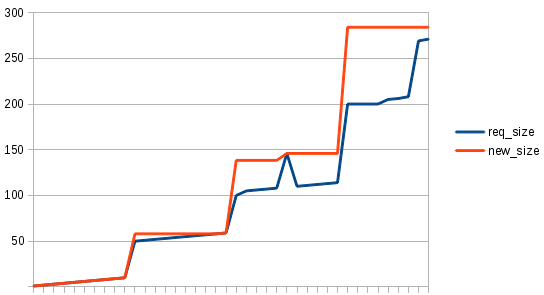
\includegraphics[width=10cm]{pics/realloc}
  \caption{New realloc method.}
  \label{figure:realloc}
\end{figure}

\input{mem/vralloc}
\chapter{Virtual Memory}

Each process owns their own master page table, in contrast to some kernels where
there might be only one master page table or one partial master page table,
and varying number of level two page tables. The kernel, also known as proc 0,
has its own master page table that is used when a process executes in kernel
mode, as well as when ever a kernel thread is executing. Static or fixed page
table entries are copied to all master page tables created. A process shares its
master page table with its childs on \verb+fork()+ while \verb+exec()+ will
trigger a creation of a new master page table.

Virtual memory is managed as virtual memory buffers (\verb+struct buf+) that
are suitable for in-kernel buffers, IO buffers as well as user space memory
mappings. Additionlly the buffer system supports copy-on-write as well as
allocator schemes where a part of the memory is stored on a secondary
storage (i.e. paging).

Due to the fact that \verb+buf+ structures are used in different allocators
there is no global knowledge of the actual state of a particular allocation,
instead each allocator should/may keep track of allocation structs if desired
so. Ideally the same struct can be reused when moving data from a secondary
storage allocator to vralloc memory (physical memory). However we
always know whether a buffer is currently in core or not (\verb+b_data+) and
we also know if a buffer can be swapped to a different allocator
(\verb+B_BUSY+ flag).

\section{Page Fault handling and VM Region virtualization}

\begin{enumerate}
\item DAB exception transfers execution to \verb+interrupt_dabt+ in \verb+XXX_int_handlers.S+
\item \verb+mmu_data_abort_handler()+ (\verb+XXX_mmu.c+) gets called
\item to be completed...
\end{enumerate}

